\section{Dataset}
\subsection{\href{https://github.com/edoardosarri24/real-time-scheduling-simulator.git}{GitHub}}

\begin{frame}{Dataset}
    \begin{columns}
        \begin{column}{.6\textwidth}
            \begin{block}{Earliest Deadline First (EDF)}
                \begin{itemize}
                    \item 5 task: 2 puramente periodici e 3 periodici.
                    \item Fattore di utilizzo di 0,95.
                    \item Chunk che campionano un additional ET da una uniforme.
                    \item \href{https://github.com/edoardosarri24/real-time-scheduling-simulator/blob/master/output/traceEDF.log}{traceEDF.log}
                \end{itemize}
            \end{block}
        \end{column}
        \begin{column}{.4\textwidth}
            \centering
            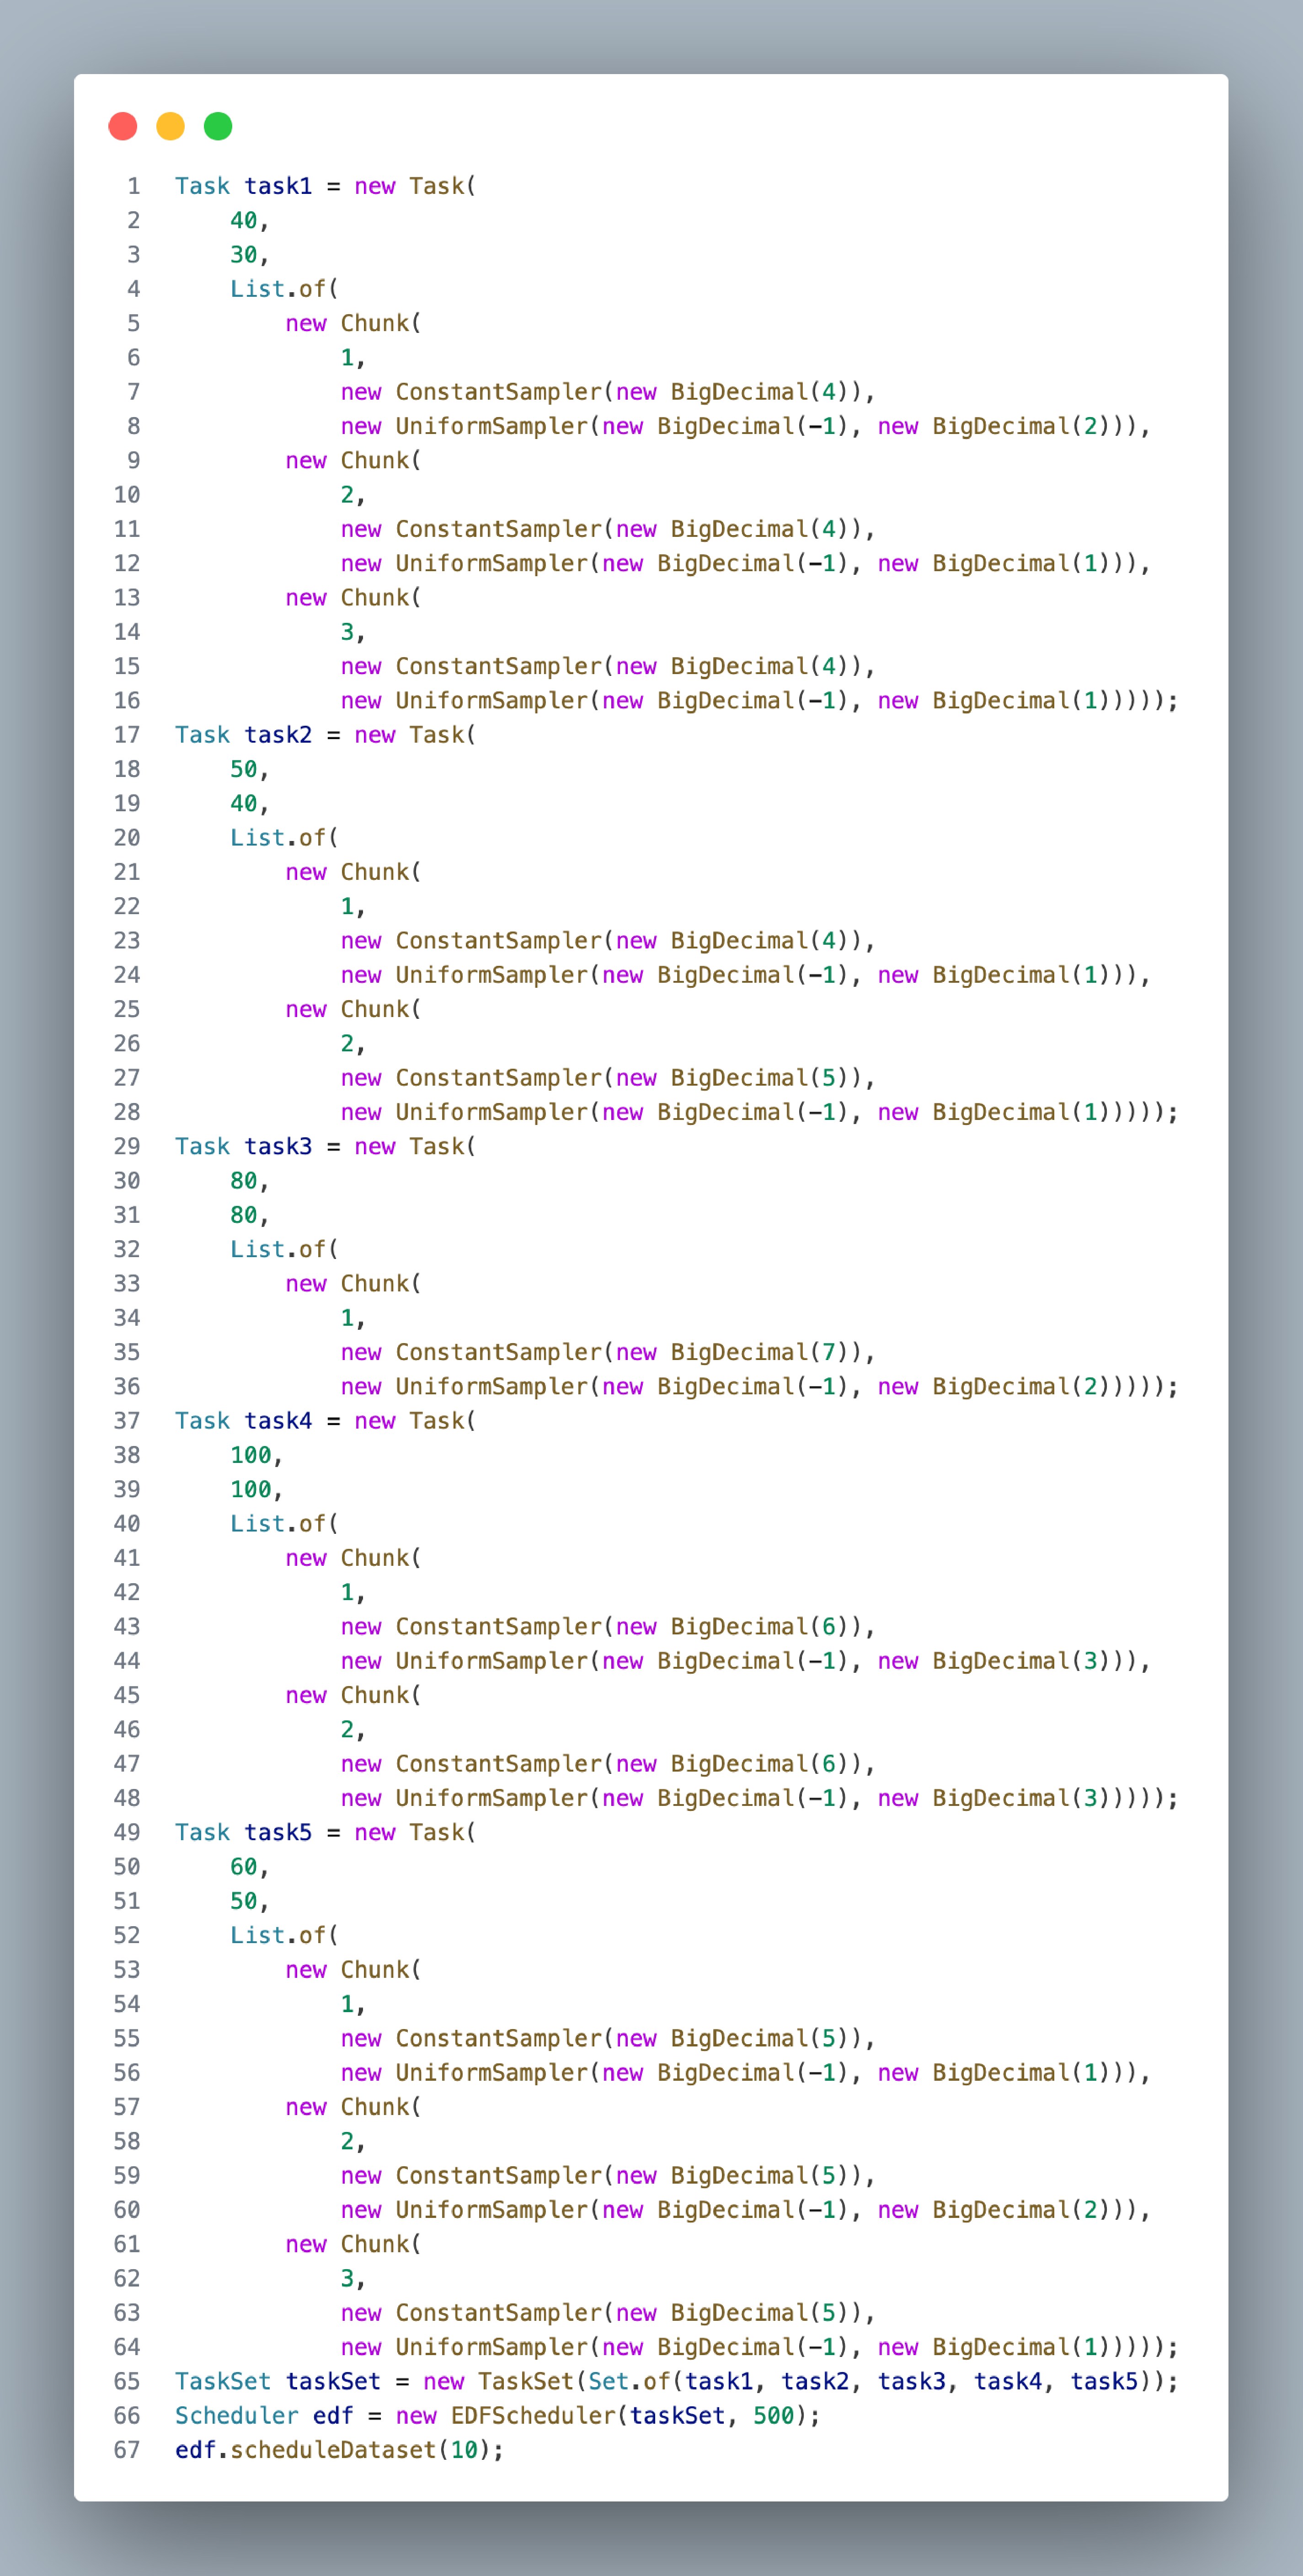
\includegraphics[width=.7\textwidth]{images/4-dataset/datasetEDF.pdf}
        \end{column}
    \end{columns}
\end{frame}

\begin{frame}{Dataset}
    \begin{columns}
        \begin{column}{.6\textwidth}
            \begin{block}{Rate Monotonic (RM)}
                \begin{itemize}
                    \item 5 task puramente periodici.
                    \item 2 risorse condivise.
                    \item Fault injection sull'acquisizione di risorse.
                    \item \href{https://github.com/edoardosarri24/real-time-scheduling-simulator/blob/master/output/traceRM.log}{traceRM.log}
                \end{itemize}
            \end{block}
        \end{column}
        \begin{column}{.4\textwidth}
            \centering
            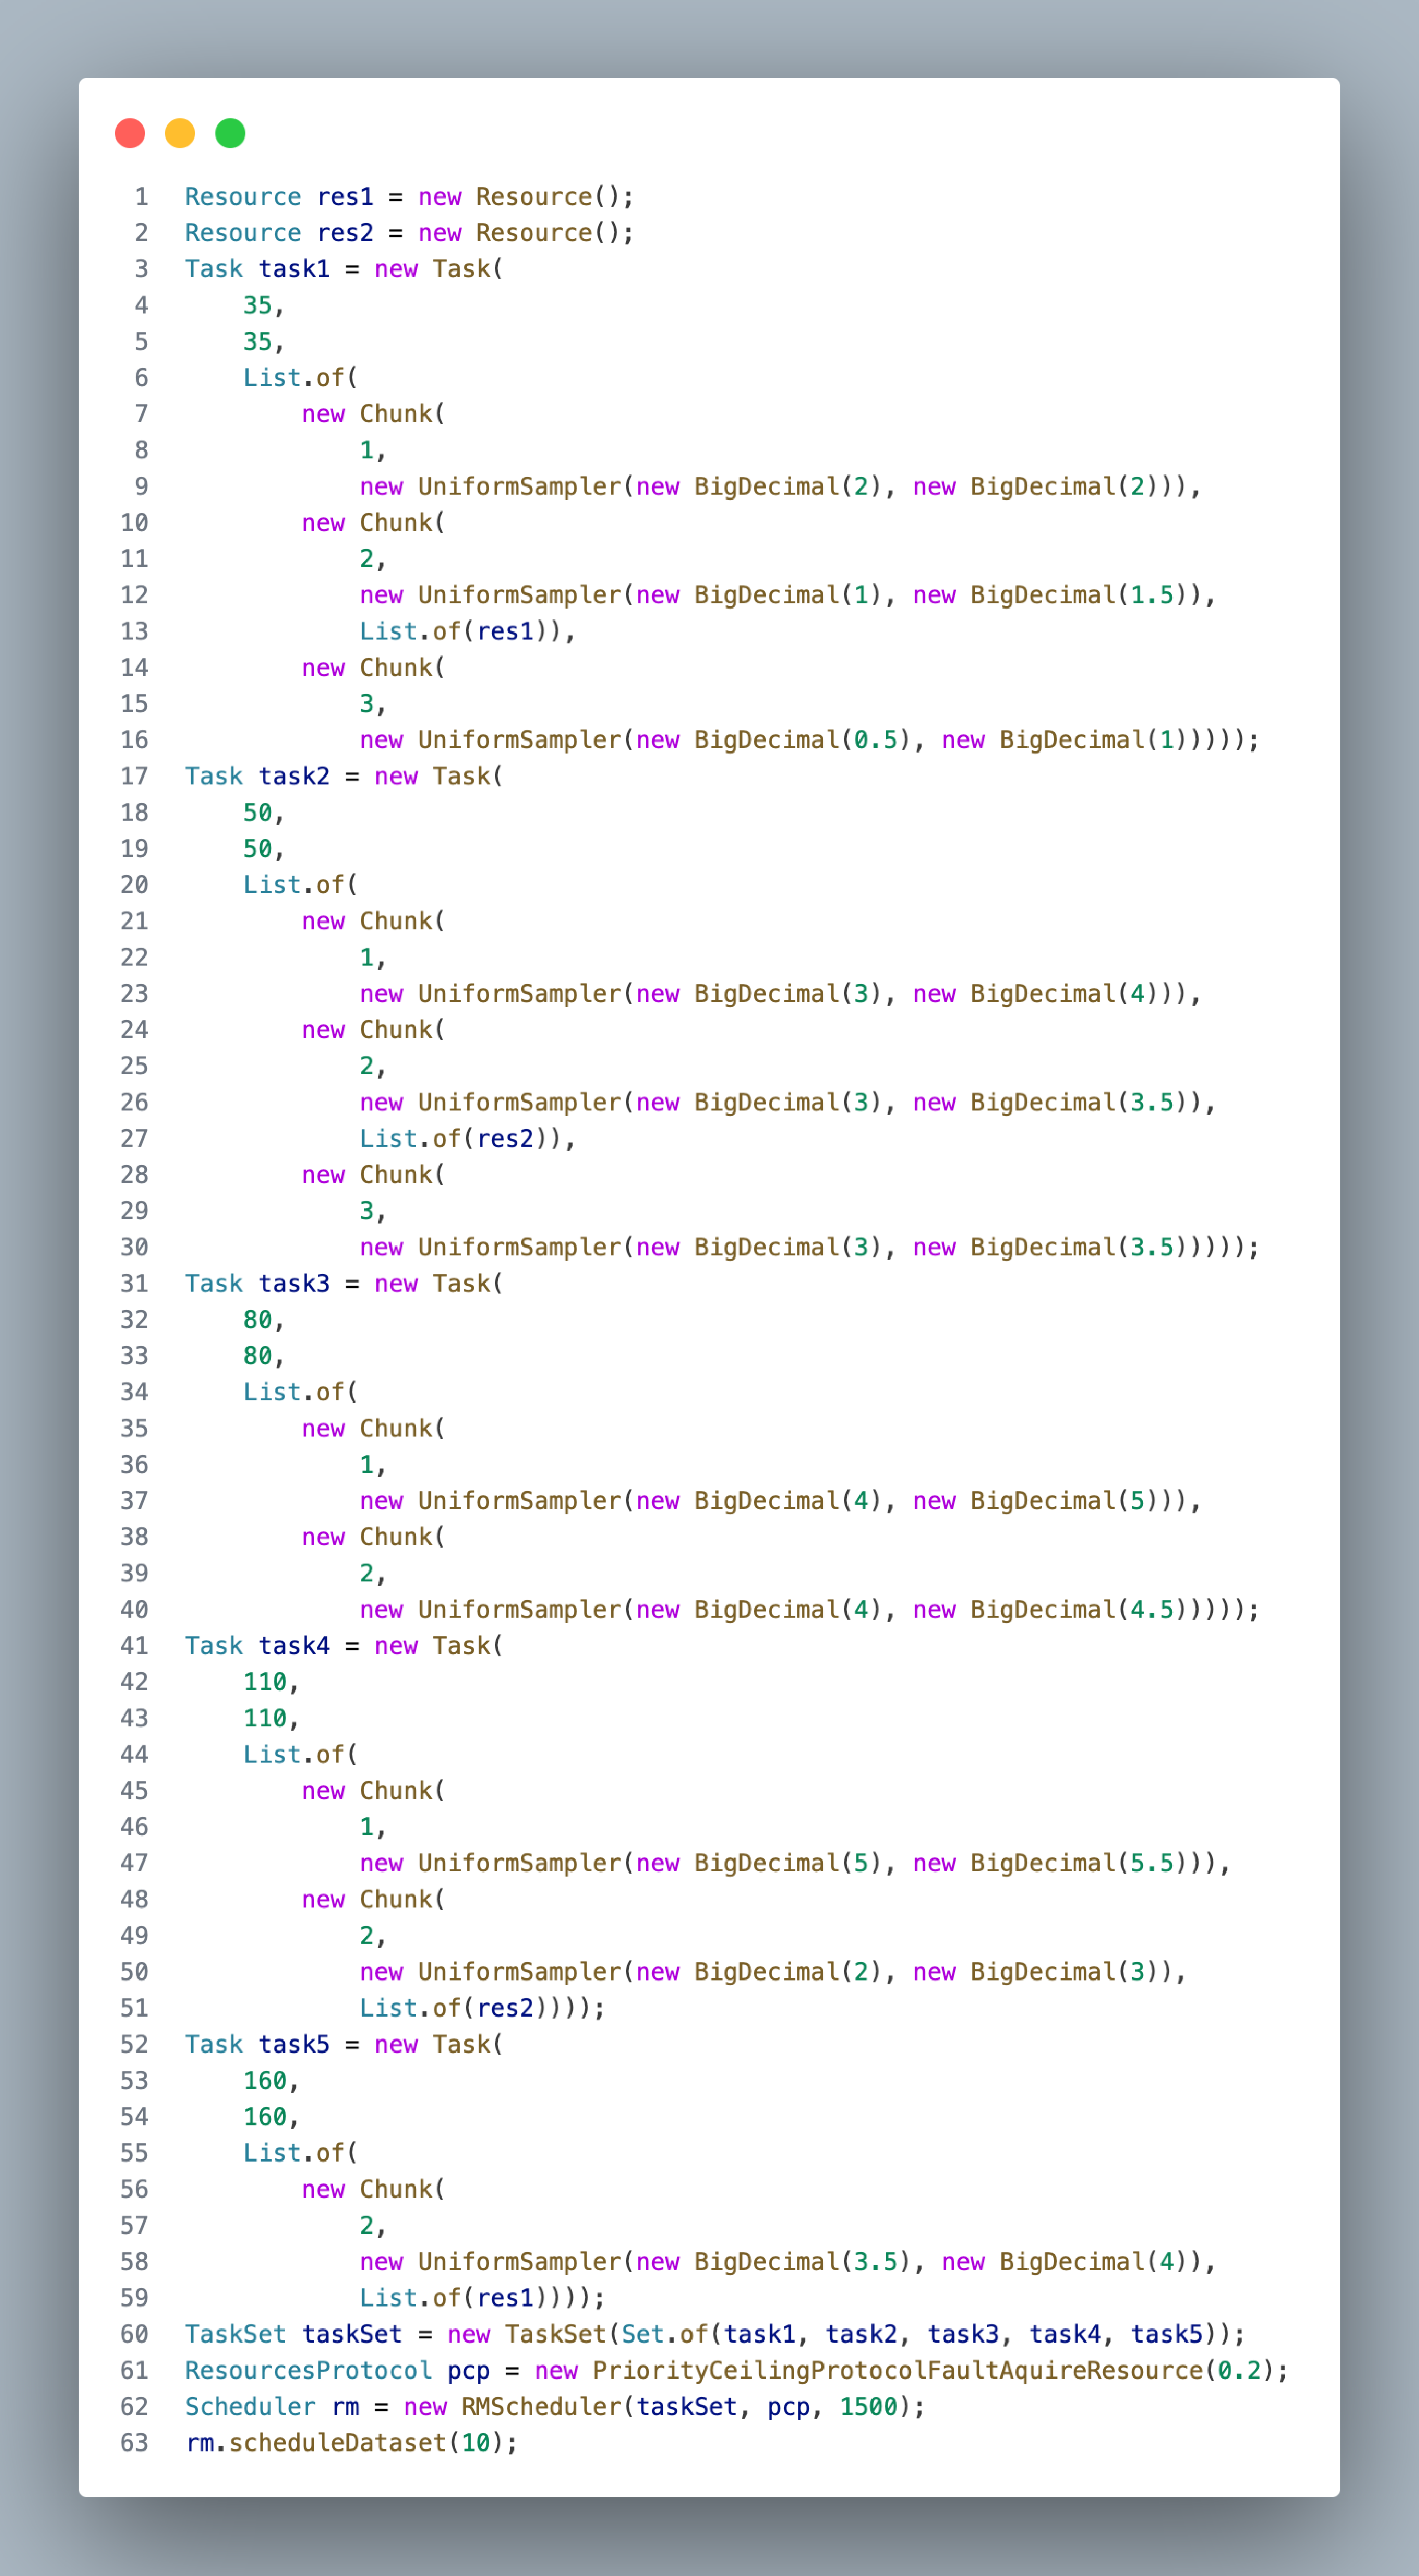
\includegraphics[width=.7\textwidth]{images/4-dataset/datasetRM.pdf}
        \end{column}
    \end{columns}
\end{frame}